\documentclass[12pt]{article}

%% Language and font encodings
\usepackage[english]{babel}
\usepackage[utf8x]{inputenc}
\usepackage[T1]{fontenc}
\usepackage{fancyhdr}

%% Sets page size and margins
\usepackage[a4paper,top=3cm,bottom=2cm,left=3cm,right=3cm,marginparwidth=1.75cm]{geometry}

%% Packages
\usepackage{xcolor}
\usepackage[colorlinks=true, allcolors=red]{hyperref}
\usepackage{lipsum}
\usepackage{graphicx}
\usepackage{float}
\usepackage[all]{hypcap}
\usepackage{changepage}
\usepackage{amsmath}
\usepackage{amssymb}
\usepackage{xspace}

%% Other
\graphicspath{{Figures/}}
\setlength\parindent{0pt}
\newcommand{\auth}{Giulia Baldini, Luis Fernandes, Agustin Vargas}
\newcommand{\ass}{Assignment 1}

%% Page settings
\pagestyle{fancy}
\fancyhf{}
\rhead{\auth}
\lhead{\ass}
\rfoot{\thepage}

\title{Foundations of Audio Signal Processing\\ \ass}
\author{\auth}

\begin{document}
	\maketitle
	\section{Complex Numbers}
	\textbf{a.}
	\begin{alignat*}{3}
		(4 − i) \cdot (2 + i) &= 8 + 4i - 2i - i^2\\
		&= 8 + 2i - (\sqrt{-1})^2\\
		&= 8 + 1 + 2i &= 9 + 2i
	\end{alignat*}
	\textbf{b.}
	\begin{alignat*}{3}
	(1 + 2i)^{-1} &= \frac{1}{(1 + 2i)} \cdot \frac{(1 - 2i)}{(1 - 2i)}\\
	&= \frac{1 - 2i}{1 - (2i)^2}\\
	&= \frac{1 - 2i}{1 + 4} &= \frac{1}{5} - \frac{2}{5} \cdot i
	\end{alignat*}
	\textbf{c.}
	\begin{alignat*}
	2 e^{2 \pi i} + e^{i \pi \frac{3}{2}} &= 2 \cdot (\cos(2 \pi) + i \cdot \sin(2\pi)) + (\cos(\frac{3}{2}\pi) + i \cdot \sin(\frac{3}{2}\pi))\\
	&= 2 \cdot (1 + 0) + (0 + i \cdot -1) &= 2 - i
	\end{alignat*}
	\textbf{d.}
	\begin{alignat*}{3}
	4 \cdot \left(\frac{1 - i}{1 + i}\right)^2 &= 4 \cdot \frac{(1 - i)^2}{(1 + i)^2}\\
	&= 4 \cdot \frac{1 -2i + i^2}{1 + 2i + i^2}\\
	&= 4 \cdot \frac{1 -2i - 1}{1 + 2i + -1}\\
	&= 4 \cdot \frac{1 -2i - 1}{1 + 2i + -1}\\
	&= 4 \cdot \frac{-2i}{2i} &= - 4 + 0 i
	\end{alignat*}
	\section{Matlab}
	\textbf{a-b.} The solutions can be found inside the \texttt{code} folder.\\
	Sample run of our program with two complex numbers:
	\begin{flushleft}
		\texttt{>> c1 = 3/4 + 2 * pi *i}\\
		\texttt{c1 = 0.75000 + 6.28319i}\\
		\texttt{>> c2 = 7 + (1/2)*i}\\
		\texttt{c2 = 7.00000 + 0.50000i}\\
		\texttt{>> Sheet1Exercise2(c1, c2)}\\
		\texttt{prod = 2.1084 + 44.3573i}\\
		\texttt{quot = 0.17039 + 0.88543i}
	\end{flushleft}
	In \autoref{plot} it is possible to see the result of our program with the above complex numbers.
	\begin{figure}[H]
	\label{plot}
	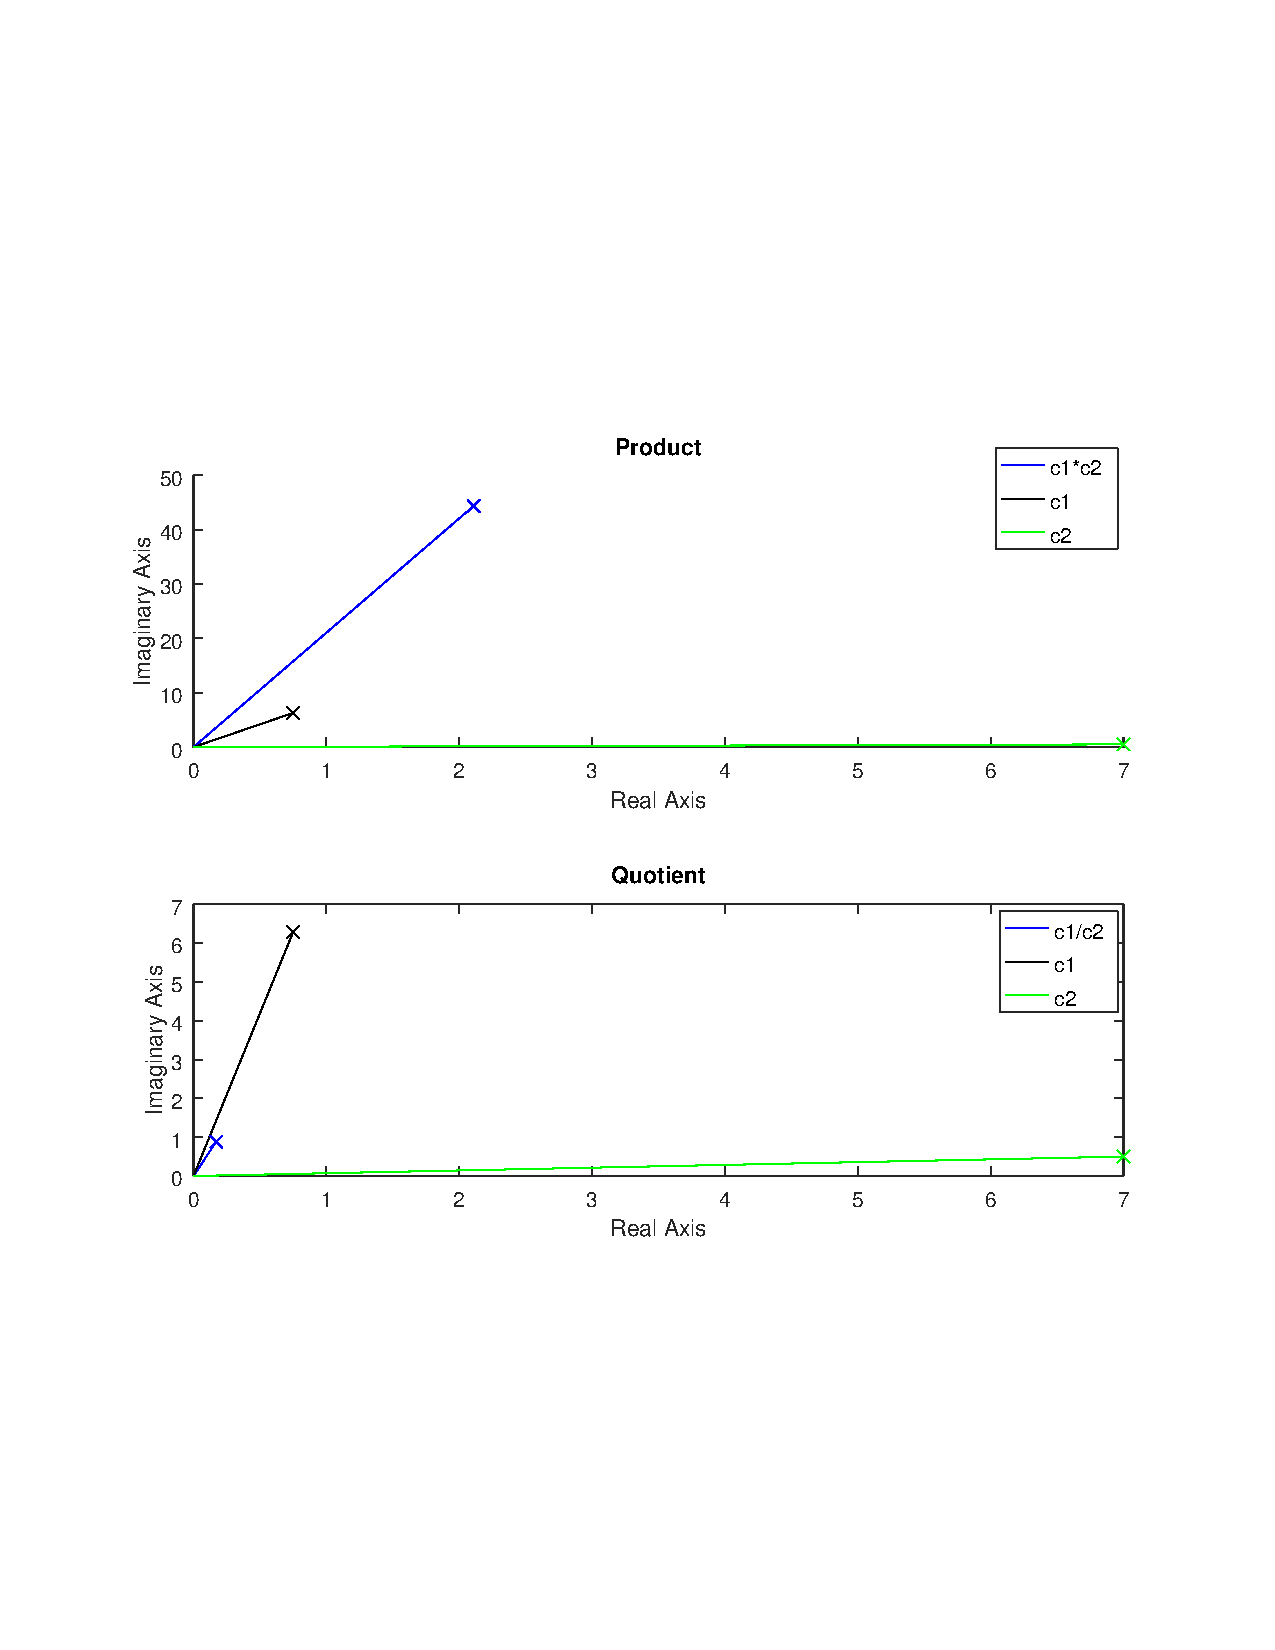
\includegraphics[width=\textwidth]{plot.pdf}
	\caption{Representations of product and quotient of two given complex numbers.}
	\end{figure}
\end{document}
